%%%
% Plantilla de Trabajo
% Modificación de una plantilla de Latex de Frits Wenneker para adaptarla 
% al castellano y a las necesidades de escribir informática y matemáticas.
%
% Editada por: Mario Román
%
% License:
% CC BY-NC-SA 3.0 (http://creativecommons.org/licenses/by-nc-sa/3.0/)
%%%

%%%%%%%%%%%%%%%%%%%%%%%%%%%%%%%%%%%%%%%%
% Short Sectioned Assignment
% LaTeX Template
% Version 1.0 (5/5/12)
%
% This template has been downloaded from:
% http://www.LaTeXTemplates.com
%
% Original author:
% Frits Wenneker (http://www.howtotex.com)
%
% License:
% CC BY-NC-SA 3.0 (http://creativecommons.org/licenses/by-nc-sa/3.0/)
%
%%%%%%%%%%%%%%%%%%%%%%%%%%%%%%%%%%%%%%%%%

%----------------------------------------------------------------------------------------
%	PAQUETES Y CONFIGURACIÓN DEL DOCUMENTO
%----------------------------------------------------------------------------------------

%%% Configuración del papel.
% fourier: Usa la fuente Adobe Utopia. (Comentando la línea usa la fuente normal)
\documentclass[paper=a4, fontsize=11pt, spanish]{scrartcl} 
\usepackage{fourier}

% Centra y formatea los títulos de sección.
% Quita la indentación de párrafos.
\usepackage{sectsty} % Allows customizing section commands
\allsectionsfont{\centering \normalfont\scshape} % Make all sections centered, the default font and small caps
\setlength\parindent{0pt} % Removes all indentation from paragraphs - comment this line for an assignment with lots of text

% Permite elegir cabeceras y pies de página.
\usepackage{fancyhdr} % Custom headers and footers
\pagestyle{fancyplain} % Makes all pages in the document conform to the custom headers and footers
\fancyhead{} % No page header - if you want one, create it in the same way as the footers below
\fancyfoot[L]{} % Empty left footer
\fancyfoot[C]{} % Empty center footer
\fancyfoot[R]{\thepage} % Page numbering for right footer
\renewcommand{\headrulewidth}{0pt} % Remove header underlines
\renewcommand{\footrulewidth}{0pt} % Remove footer underlines
\setlength{\headheight}{13.6pt} % Customize the height of the header


%%% Castellano.
% noquoting: Permite uso de comillas no españolas.
% lcroman: Permite la enumeración con numerales romanos en minúscula.
% fontenc: Usa la fuente completa para que pueda copiarse correctamente del pdf.
\usepackage[spanish,es-noquoting,es-lcroman]{babel}
\usepackage[utf8]{inputenc}
\usepackage[T1]{fontenc}
\selectlanguage{spanish}


%%% Matemáticas.
% Paquetes de la AMS. Para entornos de ecuaciones.
\usepackage{amsmath,amsfonts,amsthm}

% Incluye números entre secciones y ecuaciones.
\numberwithin{equation}{section} % Number equations within sections (i.e. 1.1, 1.2, 2.1, 2.2 instead of 1, 2, 3, 4)
\numberwithin{figure}{section} % Number figures within sections (i.e. 1.1, 1.2, 2.1, 2.2 instead of 1, 2, 3, 4)
\numberwithin{table}{section} % Number tables within sections (i.e. 1.1, 1.2, 2.1, 2.2 instead of 1, 2, 3, 4)

%%% Códigos C / C++ / SQL ...
% Paquete listings para visualización de código más elegante
\usepackage{xcolor,listings}
\usepackage{textcomp}
\lstset{upquote=true}

%% Gráficos e imagenes:
\usepackage{graphicx}


%----------------------------------------------------------------------------------------
%	TÍTULO
%----------------------------------------------------------------------------------------
% Título con las líneas horizontales, nombres y fecha.

\newcommand{\horrule}[1]{\rule{\linewidth}{#1}} % Create horizontal rule command with 1 argument of height

\title{
  \normalfont \normalsize 
  \textsc{Universidad de Granada.\\Sistemas Multidimensionales} \\ [25pt] % Your university, school and/or department name(s)
  \horrule{0.5pt} \\[0.4cm] % Thin top horizontal rule
  \huge Práctica 4: Implementación de esquemas de bases de datos multidimensionales III \\ % The assignment title
  \horrule{2pt} \\[0.5cm] % Thick bottom horizontal rule
}

\author{Daniel López García\\Rafael Nogales Vaquero} % Your name

\date{\normalsize\today} % Today's date or a custom date



%----------------------------------------------------------------------------------------
%	DOCUMENTO
%----------------------------------------------------------------------------------------


\begin{document}
\maketitle % Escribe el título
\newpage
\textbf{1. Utilizando Access, crear las tablas correspondientes a las dimensiones y a los hechos de forma que estén ligadas mediante llaves generadas.}\\
En primer lugar obtenemos de la tabla Libro la dimensión Qué 
El diseño de la consulta y el resultado obtenido se muestra en las siguientes imágenes: 
\begin{center}
	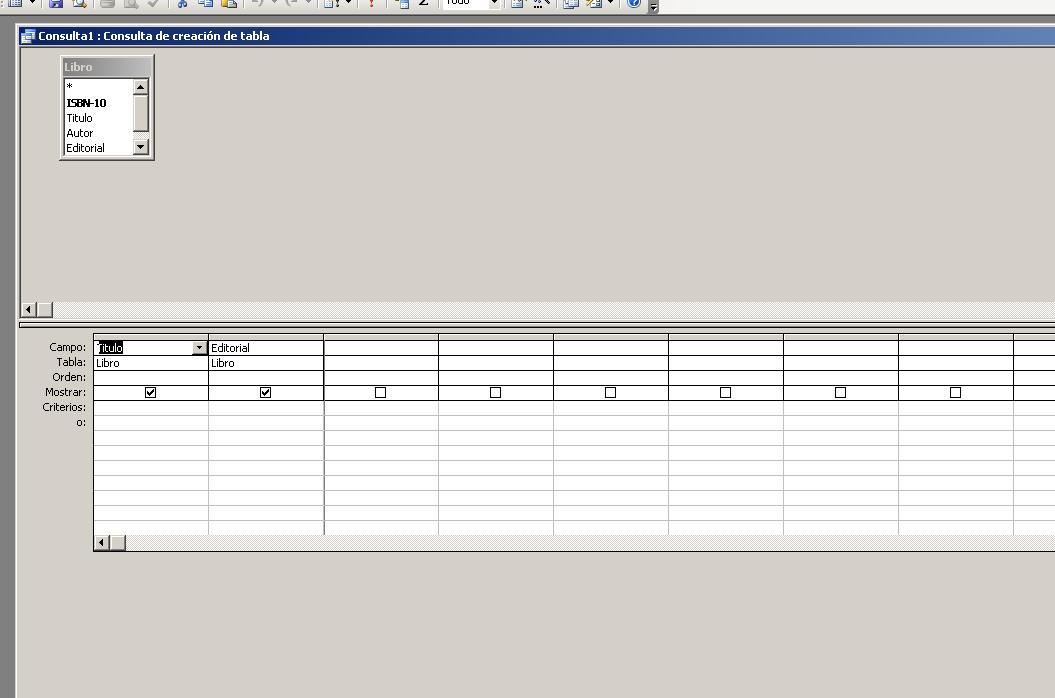
\includegraphics[]{1.JPG}
	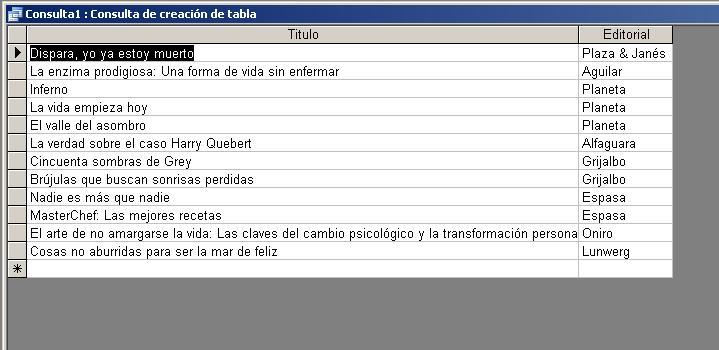
\includegraphics[]{2.JPG}
\end{center}
Una vez realizada la consulta, en la tabla creada creamos un campo autonumérico Id\_Libro.
A continuación obtenemos la tabla de la dimensión Donde a partir de la tabla Tienda.
El diseño de la consulta y el resultado obtenido se muestra en las siguientes imágenes: 
\begin{center}
	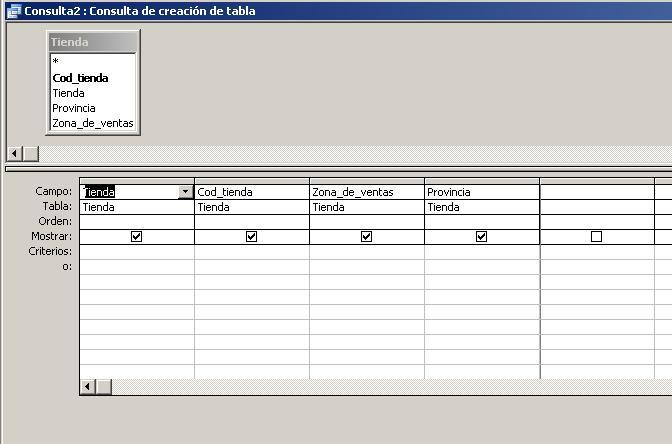
\includegraphics[scale=0.6]{3.JPG}
	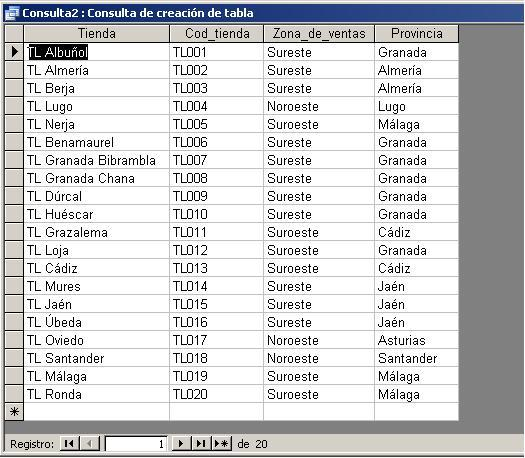
\includegraphics[scale=0.6]{4.JPG}
\end{center}
Análogamente, volvemos a crear un campo autonumérico Id\_Donde
Ahora creamos la tabla Cuando, obteniendo las fechas de la tabla LineaDeVenta y haciendo uso de las funciones Año() y Mes().
El diseño de la consulta y el resultado obtenido se muestra en las siguientes imágenes: 
\begin{center}
	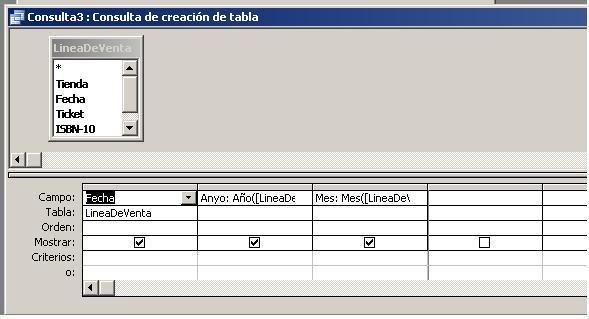
\includegraphics[scale=0.6]{5.JPG}
	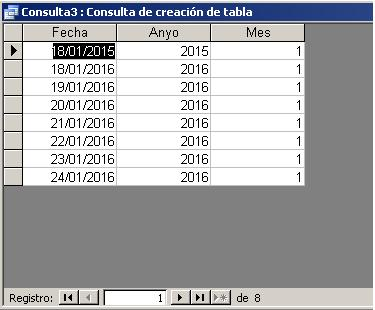
\includegraphics[scale=0.6]{6.JPG}
\end{center}
Finalmente, creamos la tabla de los hechos, Venta. Para ello usamos los campos autonuméricos creados en las tablas de las dimensiones. Para las dimensiones, hacemos uso de la tabla Libro(para obtener el PVP de cada libro) y hacemos las agregaciones necesarias.
El diseño de la consulta y el resultado obtenido se muestra en las siguientes imágenes: 
\begin{center}
	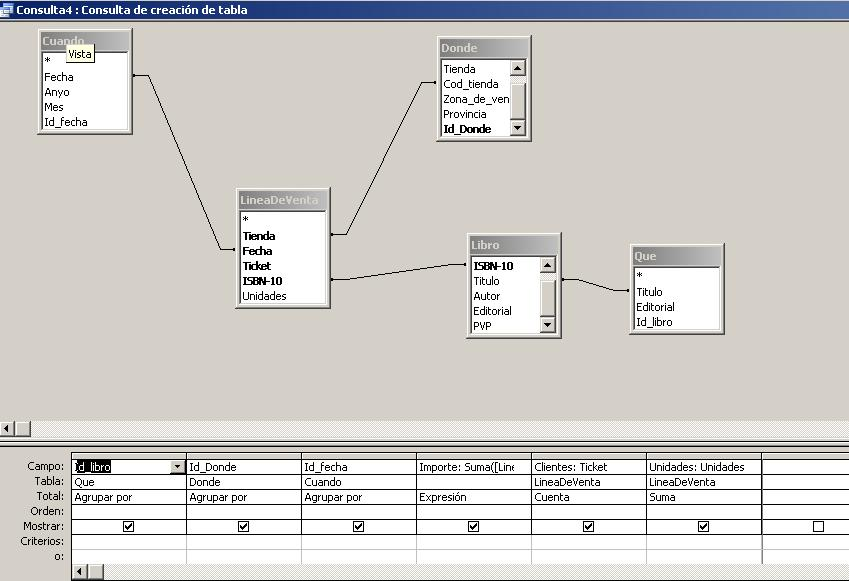
\includegraphics[scale=0.6]{7.JPG}
	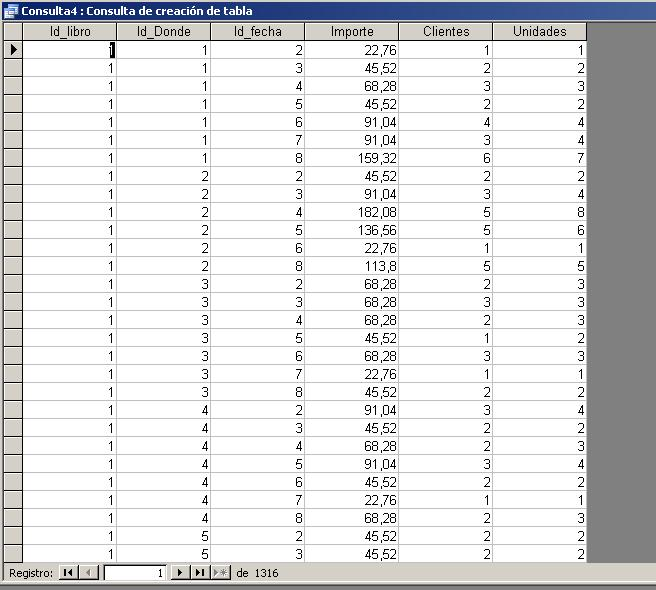
\includegraphics[scale=0.6]{8.JPG}
\end{center}
\end{document}